\chapter {Implementácia}
\todo{doplniť}

\section {Štruktúra projektu}
Implementácia webovej aplikácie začína vytvorením si základnej štruktúry projektu. S týmto môže pomôcť oficiálny nástroj pre tento účel --- \texttt{nuxi init}.

Pomocou príkazu \texttt{npx nuxi init diploma-thesis} sa vytvorí zložka \texttt{diploma-thesis}, v ktorej je možné nájsť nasledujúcu štruktúru zložiek a súborov:

\begin{figure}[H]
	\dirtree{%
		.0 diploma-thesis \DTcomment{Adresár určený pre implementáciu aplikácie}.
		.1 README.md \DTcomment{Markdown súbor obsahujúci inštrukcie pre spustenie serveru}.
		.1 app.vue \DTcomment{Vue SFC súbor obsahujúci uvítaciu správu}.
		.1 nuxt.config.ts \DTcomment{Nuxt.js konfiguračný súbor v TypeScript formáte}.
		.1 package.json \DTcomment{npm súbor obsahujúci popis projektu a jeho detaily s potrebnými balíčkami}.
		.1 public \DTcomment{Adresár určený pre verejne dostupný obsah}.
		.1 tsconfig.json \DTcomment{Konfigurácia TypeScriptu v JSON formáte}.
	}
\end{figure}

Na to, aby sa dal spustiť server s Nuxt.js frameworkom, je potrebné nainštalovať samotné balíčky tohto projektu.

\clearpage

Tieto balíčky, ktoré sú zároveň závislosťami tohto projektu, je potrebné nainštalovať príkazom \texttt{npm install}. Po ich inštalácii je už možné spustiť server, ktorý zobrazí uvítaciu správu definovanú v \texttt{app.vue} súbore.

Spustenie serveru prebehne príkazom \texttt{npm run dev}. V rámci spustenia tohto príkazu sa na konzolu vypíše adresu servera spolu s jej portom, na ktorej je možné pristúpiť k tomuto serveru. V tomto prípade sa jednalo o adresu \texttt{http://localhost:3000/}.

Čo sa týka obsahu \texttt{nuxt.config.ts} súboru, ten je spočiatku prázdny. Pomocou súboru \texttt{tsconfig.json} je možné nakonfigurovať TypeScript pre celý projekt. Jeho obsahom je referencia na \texttt{tsconfig.json} súbor samotného Nuxt frameworku --- čo znamená, že sa pre tento projekt aplikujú pravidlá TypeScriptu predvolené pre Nuxt.js projekt.

Jedným z najdôležitejších súborov v tejto štruktúre je \texttt{package.json}. Obsah tohto súboru definuje meno a detaily projektu spolu s balíčkami, ktoré sú využité v rámci samotného projektu. Popisu použitým balíčkom sa venuje nasledujúca sekcia.

\section {Použité balíčky}
V rámci tejto sekcie sú uvedené všetky balíčky, ktoré sa použili pri vývoji webovej aplikácie, z ktorých len niektoré sú nutné pre korektné fungovanie aplikácie.

Čo sa balíčkov týka, tie je možné rozdeliť na balíčky určené pre produkčné a pre vývojárske prostredie. Zmyslom tohto delenia je definovať, aké balíčky sa majú nachádzať v produkčnej zostave aplikácie. V prípade, že je balíček pridaný do sekcie vývojárskych balíčkov, nebude sa nachádzať v produkčnej zostave. Týmto krokom sa sleduje zníženie veľkosti a zrýchlenie produkčnej zostavy projektu.

\clearpage

\subsection {Balíčky pre produkčné prostredie}
\texttt{cornerstone-core} -- Balíček poskytujúci Cornerstone Core knižnicu, ktorá je zodpovedná za zobrazenie DICOM snímiek v správnom formáte a jednoduchú manipuláciu s nimi.

\texttt{@tarotoma/cornerstone-tools} -- Fork \texttt{cornerstone-tools} balíčku, ktorý obsahuje rôzne nástroje určené pre prácu s DICOM snímkami. V tomto forku bol pridaný nástroj Grid a upravená práca s prehrávaním animácií spolu s pridanými vlastnými TypeScript definíciami pre metódy používané vo webovej aplikácii, čo umožňuje lepšie našeptávanie IDE pri práci s týmto balíčkom.

\texttt{cornerstone-math} -- Tento balíček umožňuje použiť Cornerstone Math knižnicu v projekte. Tá slúži pre rôzne výpočty v oblasti vektorovej matematiky. V tomto prípade je táto knižnica potrebná len ako závislosť balíčka \texttt{@tarotoma/cornerstone-tools}.

\texttt{hammerjs} -- Účelom knižnice Hammer.js je pridanie podpory multi-dotykových gést pri práci s webovou apllikáciou. Táto funkcionalita nebola vo webovej aplikácii využitá, avšak je nutnou závislosťou balíčka \texttt{@tarotoma/cornerstone-tools}.

\texttt{dicom-parser} -- Dicom Parser je knižnica určená pre parsovanie DICOM súborov do štruktúrovaných objektov, s ktorými je možné ďalej pracovať.

\texttt{@cornerstonejs/dicom-image-loader} -- Cornerstone DICOM Image Loader a.k.a CDIL knižnica je určená pre importovanie DICOM súborov do webovej aplikácie. Táto knižnica umožňuje využiť Web Workers technológiu pre parsovanie DICOM súborov pomocou Dicom Parser knižnice.

\texttt{pinia} -- Pinia.js je knižnica určená pre tzv. state management. Umožňuje ukladať stav aplikácie tak, aby bol dostupný v rámci všetkých Vue.js komponentov. Bez použitia tejto knižnice by stavové premenné v rámci Vue.js komponentu boli dostupné len v rámci daného komponentu, jeho rodičov a potomkov.

\clearpage

Stav aplikácie je možné rozdeliť do rôznych samostatných častí pomocou modulárnych \uv{Stores}. Tie môžu byť importované nezávisle na sebe. Knižnica je taktiež plne implementovaná pomocou TypeScriptu a ponúka podporu pre konzolu prehliadača na inšpekciu aktuálneho stavu aplikácie.

\texttt{@pinia/nuxt} -- Tento balíček pridáva podporu pre integráciu Pinie do Nuxt.js.

\texttt{vuestic-ui} -- V rámci tohto projektu sa využíva Vuestic UI kit, čo je knižnica obsahujúca rôzne UI komponenty, ktoré môžu byť importované v iných projektoch. Tento UI kit bol vybraný zo subjektívneho dôvodu, nakoľko ponúka komponenty s dizajnom vhodným pre ich aplikovanie do aplikácie určenej na medicínske účely.

\texttt{@vuestic/nuxt} -- Ako už názov napovedá, tento balíček pridáva integráciu Vuestic UI do Nuxt.js aplikácie tak, aby nebola potrebná jeho ďalľia konfigurácia.

\texttt{@fortawesome/free-solid-svg-icons} -- Uvedený balíček obsahuje FontAwesome ikony, z ktorých sú niektoré použité v aplikácii v hornom paneli aplikácie.

\texttt{@fortawesome/vue-fontawesome} -- Úlohou tohto balíčka je transformovať importované FontAwesome ikony do znovupoužiteľneho komponentu, ktorý je následne možné použiť v aplikácii a pomocou neho vyrenderovať požadované ikony.

\texttt{arraybuffer-encoding} -- Tento balíček implementuje konverziu dát z \texttt{ArrayBuffer} do \texttt{base64} a naspäť. Jeho využitie je popísané neskôr v rámci kompresie odosielaných dát na server.

\texttt{crypto-random-string} -- Uvedený balíček implementuje správnu podporu generovania kryptograficky silných reťazcov. Tieto reťazce sú využívané pri anonymizácií DICOM dát pred ich odoslaním na server tak, aby nebolo možné priradiť odosielanú snímku ku konkrétnemu pacientovi.

\subsection {Balíčky pre vývojárske prostredie}
\texttt{nuxt} -- Inštalácia tohto balíčka je nutná pre vytvorenie a vývoj v rámci Nuxt.js projektu.

\texttt{eslint} -- ESLint je open-source JavaScript nástroj, ktorý kontroluje kód a reportuje prípadné nezrovnalosti v ňom. Medzi tieto nezrovnalosti partrí nekonzistentné odsadenie kódu, či používanie jazykových konštruktov, ktoré nedodržiavajú určité jednotné pravidlá. Tieto pravidlá je možné konfigurovať, ale aj importovať z iných projektov. Konfigurácia pravidiel, parsera a iných konfiguračných možností je možné pomocou \texttt{.eslintrc.cjs} súboru umiestneného v projekte.

\texttt{@typescript-eslint/parser} -- Nakoľko ESLint nepodporuje kontrolu TypeScript kódu, keďže používa Espree parser podporujúci len JavaScript, je nutné použiť tento balíček pre pridanie podpory kontroly Typescript kódu. 

\texttt{@typescript-eslint/eslint-plugin} -- Tento balíček pridáva do ESLintu pravidlá pre TypeScript kód. Použitie tohto balíčka je odporúčané prin použití predchádzajúceho balíčka.

\texttt{sass} -- Sass je CSS preprocesor, ktorý umožňuje vytvárať modulárnejší CSS kód, ktorý je jednoduchšie znovupoužiť. Okrem iného umožňuje používať CSS premenné, implementuje dedičnosť či vnáranie CSS pravidiel. Balíček \texttt{sass} implementuje Sass pomocou JavaScriptu.

\texttt{sass-loader} -- Úlohou tohto balíčka je transpilovať Sass CSS kód do čistého CSS kódu, ktorý je podporovaný CSS prehliadačmiPri budovaní projektu je nutné akýkoľvek CSS kód vytvorený pomocou Sass transpilovať do CSS, ktorý je podporovaný webovými prehliadačmi. Tento balíček v spolupráci s balíčkom \texttt{sass} konvertuje CSS kód v Sass do 

\texttt{@types/\{cornerstone-core, hammerjs, node\}} -- Tieto tri balíčky pridávajú definície typov \texttt{cornerstone-core}, \texttt{hammerjs} a \texttt{node} knižníc. Pridaním \texttt{@types} balíčkov umožňuje používať typehinty pri práci s týmito balíčkami.

\clearpage

\texttt{vue-tsc} -- Tento balíček je wrapper balíčku \texttt{tsc}, pomocou ktorého je možné transpilovať TypeScript kód do JavaScriptu. Nakoľko sa v projekte využívajú Vue SFC komponenty a samotný \texttt{tsc} balíček nepodporuje kontrolu TypeScriptu v týchto komponentách, je potrebné použiť balíček \texttt{vue-tsc} miesto \texttt{tsc} pre pridanie tejto podpory. 

\section {Inicializácia vybraných knižníc}
Biznis logika spojená s akýmkoľvek Cornerstone balíčkom a ich závislosťami bude zahrnutá v rámci súboru \texttt{Cornerstone.ts}. V ňom budú tieto balíčky importované a inicializované.

Balíčky, ktoré je nutné pred ich použitím inicializovať, sú Cornerstone Tools a Cornerstone DICOM Image Loader (CDIL). Ich inicializácia spočíva v nalinkovaní externých knižníc, ktoré dané dve knižnice využívajú v rámci ich implementácie. Bez tohto nalinkovania by niektoré metódy oboch knižníc nemuseli korektne fungovať a mohli by vyhadzovať výnimky.

Inicializácia Cornerstone Tools knižnice taktiež zahŕňa volanie metódy \texttt{init} s objektom možností, ktorú túto knižnicu pripraví pre jej použitie.

Inicializácia CDIL knižnice prebieha podobne, avšak namiesto metódy \texttt{init} sa použije metóda \texttt{configure} s objektom definujúcim jej konfiguráciu. Tá v tomto prípade zapína použitie Web Workers technológie pri parsovaní DICOM súborov. Ďalej je nutné ešte definovať konfiguráciu pracovných vlákien pomocou metódy \texttt{initialize} v rámci objektu \texttt{webWorkerManager}.

Nasledujúci kód na ďalšej strane zobrazuje popísaný import knižníc pomocou \texttt{import} až po ich inicializáciu.

\begin{minipage}[]{\linewidth}
\begin{minted}{typescript}
// Cornerstone.ts
import cornerstone from 'cornerstone-core';
import cornerstoneMath from 'cornerstone-math';
import cornerstoneTools from 'cornerstone-tools';
import cornerstoneDICOMImageLoader from '@cornerstonejs/dicom-image-loader';
import dicomParser from 'dicom-parser';
import Hammer from 'hammerjs';

/**
 * Initialize cornerstone libraries
 */
export const initLibraries = (): void => {
  // Setup all required cornerstone-tools dependencies
  cornerstoneTools.external.cornerstone = cornerstone;
  cornerstoneTools.external.cornerstoneMath = cornerstoneMath;
  cornerstoneTools.external.Hammer = Hammer;
  cornerstoneTools.init({
    mouseEnabled: true,
    showSVGCursors: false,
  });

  // Setup all required cornerstone-wado-image-loader dependencies
  cornerstoneDICOMImageLoader.external.cornerstone = cornerstone;
  cornerstoneDICOMImageLoader.external.dicomParser = dicomParser;
  cornerstoneDICOMImageLoader.configure({
    useWebWorkers: true,
    decodeConfig: {
      convertFloatPixelDataToInt: false,
    },
  });

  const config = {
    maxWebWorkers: navigator.hardwareConcurrency || 1,
    startWebWorkersOnDemand: false,
    taskConfiguration: {
      decodeTask: {
        initializeCodecsOnStartup: true,
        strict: false,
      },
    },
  };
  cornerstoneDICOMImageLoader.webWorkerManager.initialize(config);
}
\end{minted}
\end{minipage}

\section {Štruktúra komponentov používateľského rozhrania}
Po inicializácii projektu, inštalácii knižníc a ich inicializácii je nutné zamyslieť sa nad štruktúrou samotných Vue komponentov, ktoré budú definovať používateľské rozhranie webovej aplikácie.

Keďže návrhu používateľského prostredia vyplýva, že bude rozdelený na 4 hlavné časti, ponúka sa možnosť rozdeliť potrebné komponenty taktiež do 4 zložiek. Tými budú \texttt{top-panel}, \texttt{left-panel}, \texttt{main-window} a \texttt{right-panel}. Komponenty použité v rámci jednej časti používateľského rozhrania budú spadať do danej zložky. Akýkoľvek komponent použitý vo viacerých častiach by mal byť umiestnený v zložke \texttt{general}.

Pre každú časť tohto rozhrania by mal byť taktiež vytvorený jeden hlavný komponent reprezentujúci danú časť aplikácie. Nakoľko tieto komponenty nebudú znovupoužiteľné, ich prefixom musí byť člen \uv{The} podľa Vue.js konvencií. Jedná sa o nasledujúce komponenty: \texttt{TheTopPanel.vue}, \texttt{TheLeftPanel.vue}, \texttt{TheMainWindow.vue} a \texttt{TheRightPanel.vue}.

Tie budú importované v jednom entry-point komponente, ktorý bude definovať hlavnú (a jedinú) stránku aplikácie. Tento komponent bude niesť názov \texttt{index.vue} a bude umiestnený v priečinku \texttt{pages}, aby Nuxt.js spároval zobrazenie tohto komponentu pri požadovanej návšteve indexovej stránky. V tomto komponente bude taktiež importovaná metóda \texttt{initLibraries} uvedená v predchádzajúcej časti kódu. Tá bude exekuovaná v rámci metódy \texttt{onMounted}, ktorá zaručuje exekúciu kódu po tom, čo je používateľské rozhranie súčasťou Document Object Modelu (DOM) webovej aplikácie.

\clearpage

Výsledná štruktúra pre definovanie častí UI a ich komponentov je nasledujúca:
\begin{figure}[H]
	\dirtree{%
                 .0 diploma-thesis \DTcomment{Adresár určený pre implementáciu aplikácie}.
                 .1 components \DTcomment{Adresár určený pre komponenty}.
		.2 top-panel \DTcomment{Adresár pre komponenty použité v hornom paneli}.
		.2 left-panel \DTcomment{Adresár pre komponenty použité v ľavom paneli}.
		.2 main-window \DTcomment{Adresár pre komponenty použité v centrálnej časti aplikácie}.
		.2 right-panel \DTcomment{Adresár pre komponenty použité v pravom paneli}.
		.2 general \DTcomment{Adresár pre komponenty použité vo viacerých častiach aplikácie}.
		.2 TheTopPanel.vue \DTcomment{Vue SFC komponent reprezentujúci horný panel}.
		.2 TheLeftPanel.vue \DTcomment{Vue SFC komponent reprezentujúci ľavý panel}.
		.2 TheMainWindow.vue \DTcomment{Vue SFC komponent reprezentujúci centrálnu časť aplikácie}.
		.2 TheRightPanel.vue \DTcomment{Vue SFC komponent reprezentujúci pravý panel}.
		.1 pages \DTcomment {Adresár obsahujúci stránky aplikácie}.
		.2 index.vue \DTcomment {Vue SFC komponent reprezentujúci index stránku aplikácie}.
	}
\end{figure}

\section{Implementácia prípadov použitia}
Poradie implementácie prípadov použitia dáva zmysel v poradí, v akom boli uvedené. T.j. ako prvé bude implementované zobrazenie snímiek vo webovej aplikácii. \todo{dokončiť}

\subsection {UC1 -- Zobrazenie snímiek v aplikácii}
V rámci tohto prípadu použitia je nutné implementovať import snímiek a ich zobrazenie vo webovej aplikácii.

Pred samotným importom snímiek je potrebné označiť vybraný HTML element pomocou Cornerstone Core knižnice. Označenie tohto elementu spočíva v zavolaní statickej metódy \texttt{enable}, ktorej argumentom je daný element. V takto označenom elemente sa budú zobrazovať snímky z magnetickej rezonancie. Následne je možné pristúpiť k importu DICOM snímiek.

Import DICOM snímiek sa dá realizovať pomocou tlačidla, ktoré bude naviazané na File API, ktoré je poskytované prehliadačmi a umožňuje načítať rôzne súbory do pamäti prehliadača. Následne bude potrebné tieto súbory sparsovať, aby bolo možné s nimi ďalej pracovať.

Parsovanie importovaných DICOM snímiek je možné dosiahnuť pomocou CDIL knižnice. Následne je nutné použiť knižnicu Cornerstone Core pre načítanie týchto snímiek do internej cache. To zaručí, že sa pri neskoršom zobrazovaní snímiek nemusia tieto snímky znovu načítavať, čo zvyšuje používateľský komfort pri používaní aplikácie.

Následne je možné použiť statickú metódu \texttt{displayImage} Cornerstone Core knižnice pre zobrazenie MR snímky. Tá bude vykreslená vo zvolenom označenom HTML elemente.

Bližší pohľad na algoritmus zodpovedný za import snímiek, ich parsovanie až po výsledné zobrazenie je možné vidieť na nasledujúcom sekvenčnom diagrame.

\begin {center}
        \centering
        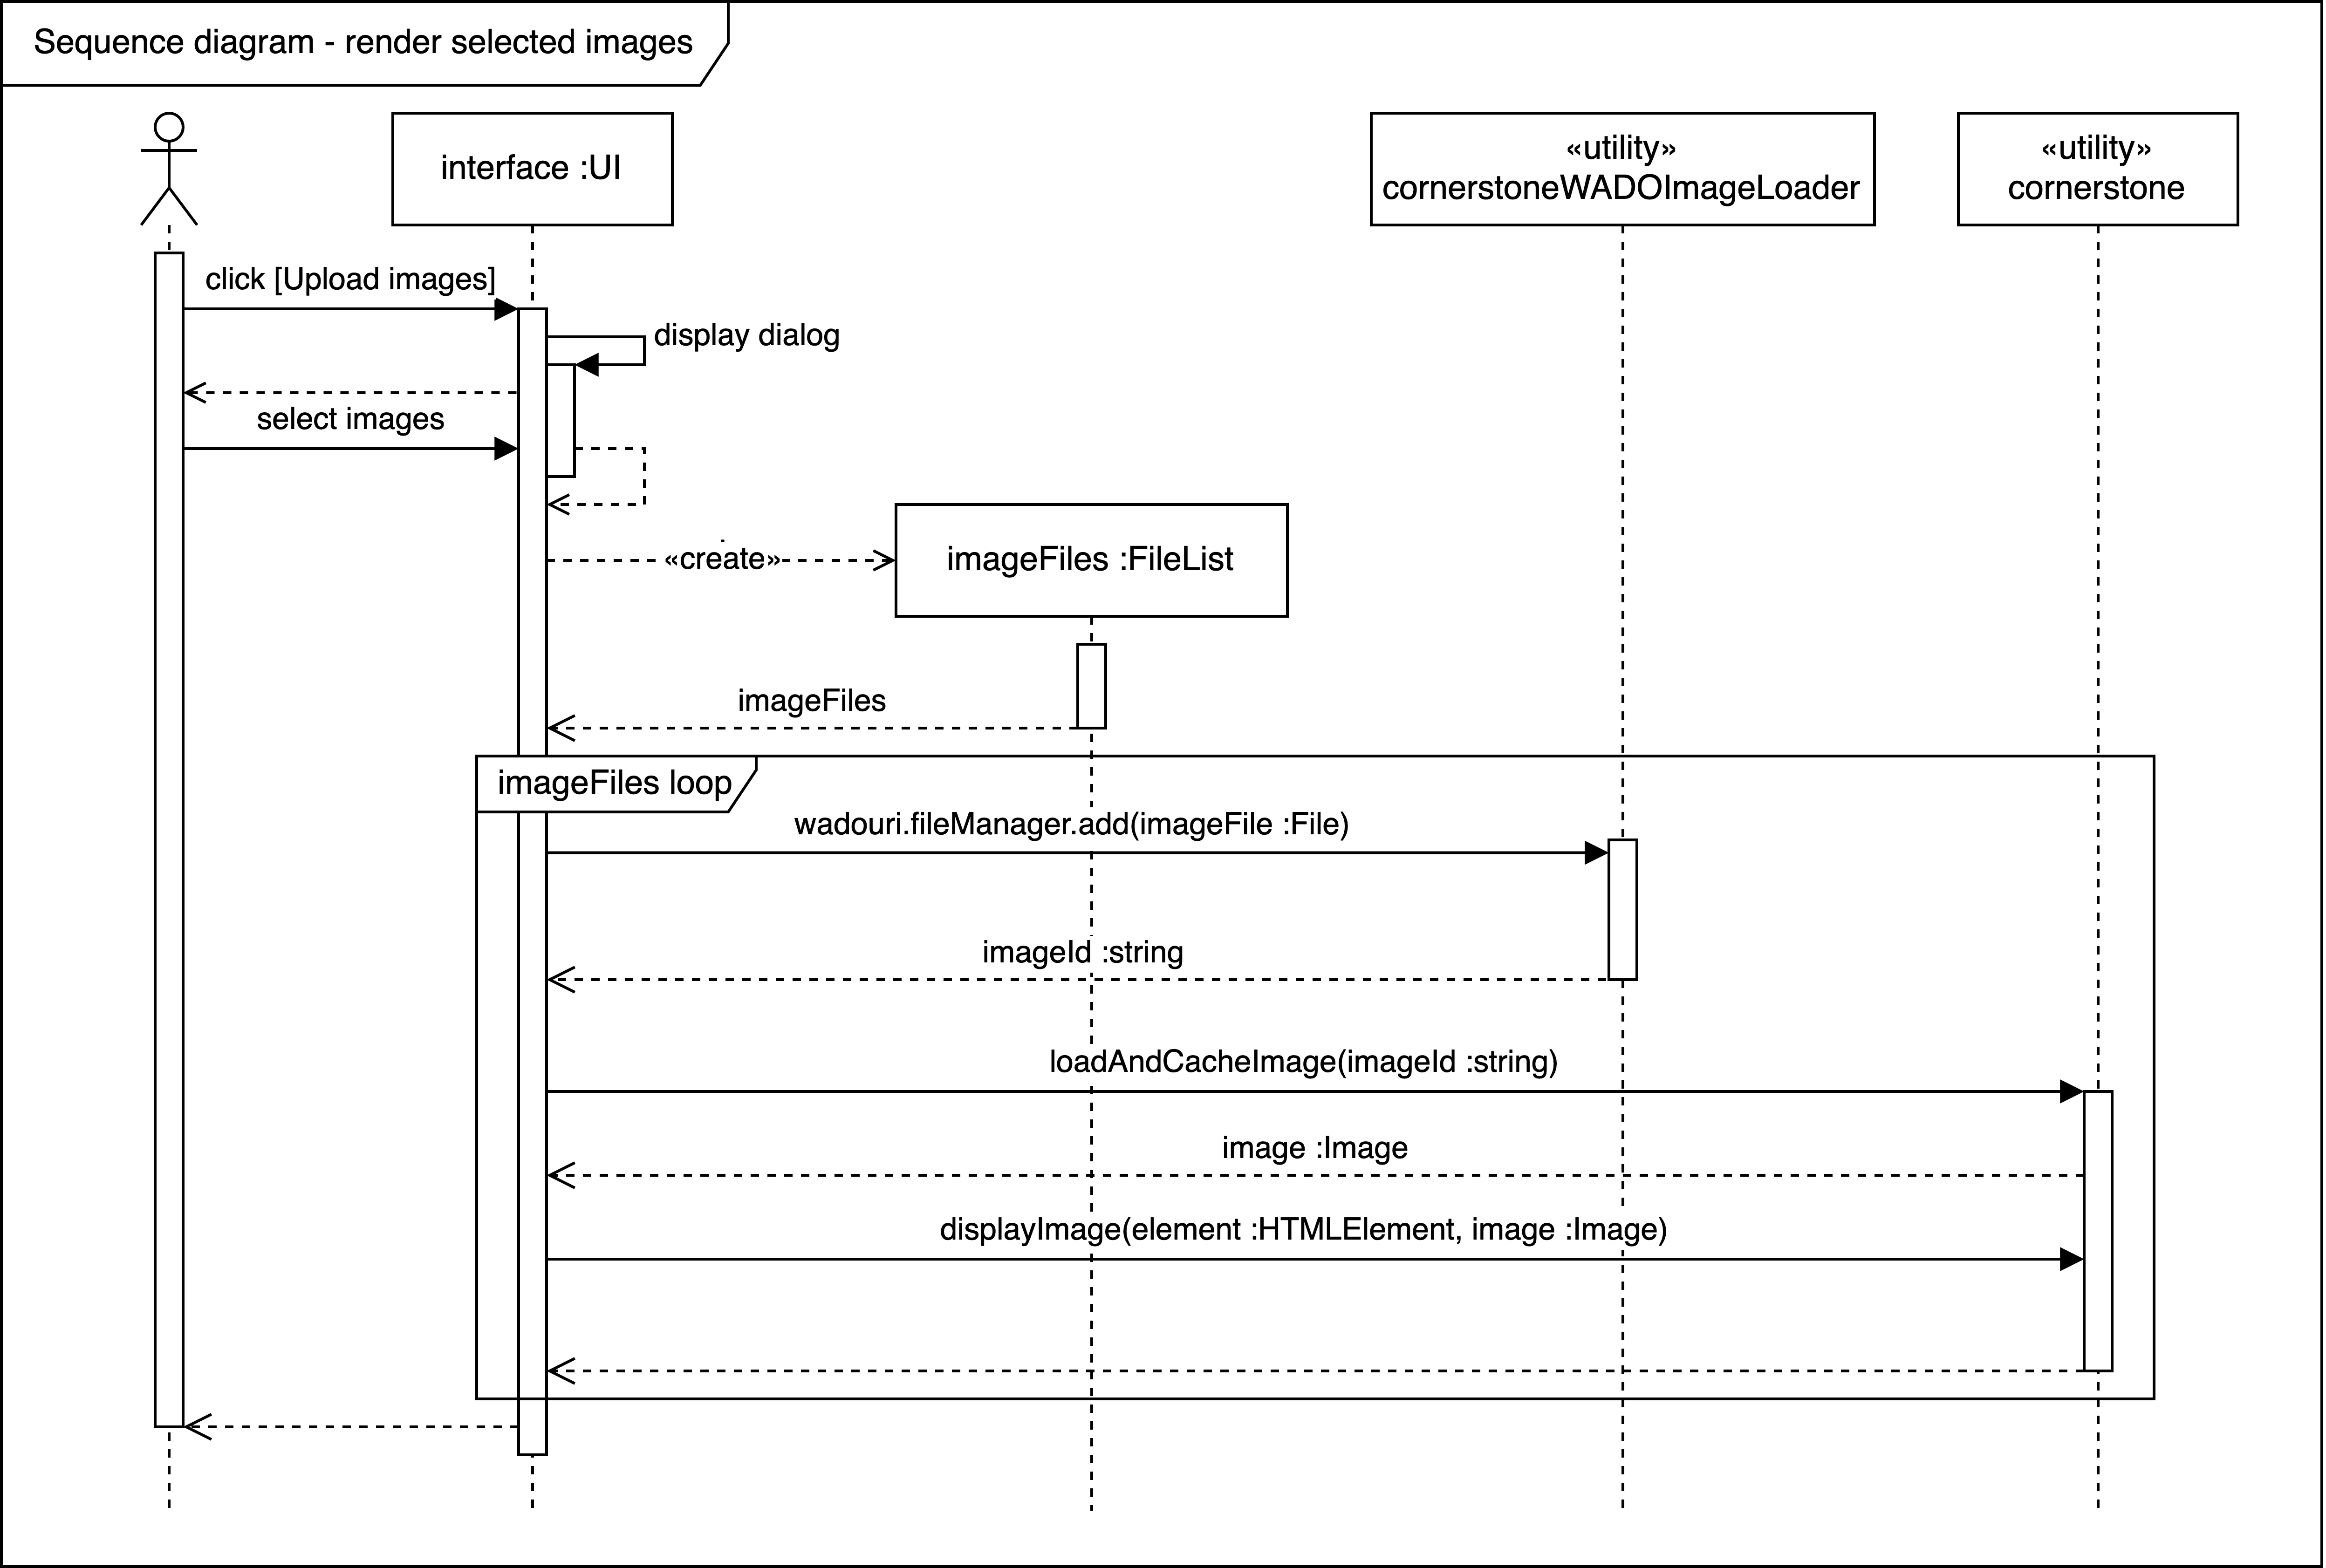
\includegraphics[height=9cm]{media/graphs/render_images.png}
        \captionsetup{justification=centering}
        \captionof{figure}{Sekvenčný diagram zobrazujúci import, parsovanie a zobrazenie DICOM snímiek}
\end {center}

\subsection {UC2 -- Animácia snímiek}
Knižnica Cornerstone Tools ponúka nástroj \uv{PlayClip}, pomocou ktorého je možné importované snímky animovať. Avšak po bližšej analýze tohto nástroja bolo zistené, že nie je konfigurovateľný do takej miery, ako vyžaduje alternatívny scenár tohto prípadu použitia. PlayClip nástroj neprijíma indexy snímiek ako argumenty, od akej, resp. po akú snímku sa animácia má prehrávať.

\subsubsection {Vytvorenie a publikácia forku Cornerstone Tools knižnice}
Táto skutočnosť viedla k potrebe vytvorenia vlastného forku Cornerstone Tools knižnice za účelom zmeny \uv{PlayClip} nástroja. Algoritmus tohto nástroja - metóda \texttt{playClip} -- bola zmenená tak, aby prijímala chýbajúce argumenty a na ich základe animovala snímky. Pomocou metódy \texttt{stopClip} je možné prebiehajúcu animáciu zastaviť.

Takto upravená knižnica bola publikovaná do npm registru pod názvom \texttt{@tarotoma/cornerstone-tools}. Pre použitie upravenej knižnice v projekte je nutné zmazať existujúcu knižnicu a nahradiť ju jej forknutou verziou. 

Na to, aby mohol \uv{PlayClip} nástroj korektne fungovať, je potrebné ho pridať spolu s nástrojom \texttt{stack} do tzv. \uv{Stack stratégie manažovania stavu nástrojov}. K stavu nástrojov spravovaných touto stratégiou je možné pristupovať z akejkoľvek snímky. Predvolene je stav nástrojov oddelený pre každú snímku, nakoľko je pri väčšine nástrojov žiaduce mať zobrazené informácie viažuce sa k danej snímke.

Okrem úpravy \uv{PlayClip} nástroja boli taktiež vytvorené TypeScript definície typov pre metódy používané webovou aplikáciou.

\subsection {UC3 -- Vytvorenie mriežky}
Vykreslenie mriežky nad zobrazenou snímkou patrí medzi hlavné funkčné požiadavky kladené na túto aplikáciu. Nakoľko Cornerstone Tools knižnica neposkytuje taký nástroj, bude potrebné ho vytvoriť. Keďže je v projekte už použitý fork Cornerstone Tools knižnice, je priamočiarejšie implementovať tento nástroj rovno v rámci neho.

Cieľom implementácie nového nástroja je umožniť používateľovi webovej aplikácie vykresliť nad zobrazenou DICOM snímkou mriežku, ktorá by bola parametrizovateľná používateľom. Na základe týchto parametrov by sa mala mriežka vykresliť v požadovanej podobe.

Pred začatím implementácie nástroja mriežky je dôležité zoznámiť sa s anatómiou Cornerstone Tools nástrojov, ktorej sa venujú nasledujúce podsekcie. a dostupných informácií na stránke projektu a API dokumentáciu Cornerstone Tools knižnice. \todo{stranka projektu}

\subsubsection {Dostupné módy nástrojov}
Cornerstone Tools nástroje sa môžu nachádzať v štyroch rôznych módoch, z ktorého je vždy jeden mód aplikovaný. Na základe práve aktívneho módu môže byť nástroju deaktivovaná rozličná funkcionalita.

Zoznam dostupných módov je nasledovný:
\begin {itemize}
\item {aktívny mód,}
\item {pasívny mód,}
\item {zapnutý mód a}
\item {vypnutý mód.}
\end {itemize}

Ak je nástroj v aktívnom móde, je mu umožnené zobraziť jeho obsah a meniť svoj vnútorný stav. Nástroj v tomto stave môže tiež reagovať na interakciu používateľa s týmto nástrojom.

Narozdiel od aktívneho módu, pasívny mód umožňuje všetko čo aktívny mód s tým rozdielom, že nie je možné vytvoriť nový stav nástroja, ale len manipulovať s jeho existujúcim stavom.

Nástroje v zapnutom móde je možné vyrenderovať, avšak nereagujú na interakciu používateľa s takýmto nástrojom. Jedná sa vlastne o taký \uv{read-only} mód nástroja.

Vypnutý mód nástroja narozdiel od všetkých uvedených módov neumožňuje s takýmto nástrojom interagovať a ani tento nástroj vykresliť. Tento mód je taktiež predvoleným módom pre každý nástroj. \todo{citacia}

Použitie vybraného nástroja je možné až po jeho registrácii. Nasledujúca metóda \texttt{registerTool} implementuje registráciu a nastavenie zapnutého módu registrovaného nástroja.
\begin{minted}{typescript}
export const registerTool = (toolName: cornerstoneTools.ToolName): void => {
  const store = useGlobalStore() // store retrieval
  if (!store.mainImageContainer) {
    return
  }
  const fullToolName = toolName + 'Tool' as cornerstoneTools.FullToolName
  const tool = cornerstoneTools[fullToolName]
  cornerstoneTools.addToolForElement(store.mainImageContainer, tool)
  cornerstoneTools.setToolEnabledForElement(store.mainImageContainer, toolName)
}
\end{minted}

\todo{presunut tento kod do registracie nastroja co bude po vytvoreny }

\subsubsection {Popis triedy mriežky a jej metód}
Pomocou Cornerstone Tools knižnice je možné vytvoriť tri typy nástrojov -- pre implementáciu nástroja mriežky je vhodné vychádzať z tzv. \uv{Base Annotation} nástroja. Takýto nástroj umožňuje vytvárať a manipulovať s anotáciami snímiek.

Trieda tohto typu nástroja -- \texttt{BaseAnnotationTool} rozširuje triedu \texttt{BaseTool}, ktorá je základnou triedou pre všetky implementované nástroje.

\texttt{BaseTool} trieda je zodpovedná za inicializáciu konfigurácie nástroja, dynamické aplikovanie dodatočnej funkcionality a virtuálne funkcie pre interakciu s nástrojom pomocou myši alebo dotyku. \todo{pridat citaciu} Poskytované virtuálne funkcie sú nasledovné:
\begin {itemize}
\item {\texttt{preMouseDownCallback},}
\item {\texttt{postMouseDownCallback},}
\item {\texttt{preTouchStartCallback} a}
\item {\texttt{postTouchStartCallback}.}
\end {itemize}

\texttt{preMouseDownCallback} je funkcia, ktorá je spustená pred tým, ako sa začne spracovávať \texttt{mousedown} event. Predvolene táto callback funkcia nerobí nič.
\texttt{postMouseDownCallback} je funkcia, ktorá je spustená po spracovaní \texttt{mousedown} eventu. Predvolene taktiež nič nerobí.

Posledné dve funkcie -- \texttt{preTouchStartCallback} a \texttt{postTouchStartCallback} sú funkcie, ktoré sú funkcionalitou podobné funkciám \texttt{preMouseDownCallback} a \texttt{postMouseDownCallback}. Rozdiel medzi nimi je ten, že zatiaľ čo prvé dve reagujú na stlačenie tlačidla myši (\texttt{mousedown} event), posledné dve reagujú na dotyk dotykovej plochy (\texttt{touchstart} event).

BaseAnnotationTool trieda rozširuje počet virtuálnych metód o nasledujúce 4 metódy:
\begin {itemize}
\item {\texttt{mouseMoveCallback},}
\item {\texttt{handleSelectedCallback},}
\item {\texttt{toolSelectedCallback} a}
\item {\texttt{updateCachedStats}.}
\end {itemize}

\texttt{mouseMoveCallback} je funkcia, ktorá sa spustí pri detekcii \texttt{mousemove} eventu. Ten je spúšťaný prehliadačom počas každého pohybu myšou.
\texttt{handleSelectedCallback} je taktiež funkcia, ktorá sa avšak spúšťa po zvolení časti vykreslenej anotácie myšou alebo dotykom.
\texttt{toolSelectedCallback} je funkcia, ktorá sa spustí pri zvolení daného nástroja.
\texttt{updateCachedStats} funkcia je zodpovedná za aktualizáciou štatistík daného nástroja.

Nakoľko sú všetky spomenuté metódy virtuálne, nemusia byť koniec koncov daným nástrojom implementované.
Avšak \texttt{BaseAnnotationTool} trieda poskytuje aj abstraktné metódy, ktoré je nutné implementovať. Ich zoznam je nasledovný:
\begin {itemize}
\item {\texttt{createNewMeasurement},}
\item {\texttt{pointNearTool},}
\item {\texttt{distanceFromPoint} a}
\item {\texttt{renderToolData}.}
\end {itemize}

\texttt{createNewMeasurement} metóda je zodpovedná za vytvorenie novej anotácie a jej uloženie do pamäte. Táto metóda sa exekuuje v rámci práve aktívneho nástroja ak žiaden nástroj neodpovedal na \texttt{mousedown} event.
Metóda \texttt{pointNearTool} vráti pravdivú hodnotu, ak koordináty kliknutia myšou alebo dotyku na dotykovú plochu sa nachádzajú blízko anotácie nástroja. Ak áno, tak daná časť anotácie je poslaná ako argument \texttt{toolSelectedCallback} metódy.
\texttt{distanceFromPoint} metóda vracia počet pixelov medzi zadanou súradnicou a najbližšou časťou anotácie.
V rámci metódy \texttt{renderToolData} je nutné implementovať vykreslenie anotácie na snímku. Samotné vykreslenie sa dá dosiahnuť pomocou interných metód ako \texttt{drawJoinedLines} pre vykreslenie úsečiek spojených v určitých bodoch či \texttt{drawHandles} pre vykreslenie bodov, ktoré môžu byť presúvané po ploche snímky.

\subsubsection {Manažment stavu mriežky}
Stav nástrojov je možné uložiť a získať pomocou metód \texttt{addToolState} a \texttt{getToolState} po ich importovaní z \texttt{stateManagement/toolState.js} súbora.

Stav mriežky bude reprezentovaný poľom obsahujúcim štruktúru vertikálnych úsečiek. Jedna takáto úsečka bude predstavovať tzv. measurement. V rámci mriežky budú uložené body tejto úsečky. Tá bude obsahovať $x$ a $y$ koordináty bodu spolu s príznakom, či je daný bod hlavným (common) bodom alebo tzv. \uv{refinement} bodom. 
Postupnosť uložených bodov bude predstavovať vertikálnu úsečku. Horizontálne úsečky budú automaticky dopočítané pri renderovaní mriežky pomocou susedných bodov priľahlých vertikálnych úsečiek.

Z horeuvedeného vyplýva, že pri volaní metódy \texttt{createNewMeasurement} sa x-krát reprezentácia vertikálnych úsečiek, ktoré budú v cykle ukladané do celkového stavu mriežky pomocou metódy \texttt{addToolState}.

Reprezentácia vertikálnej úsečky bude teda vyzerať nasledovne:
\begin{minted}[autogobble,bgcolor=white]{typescript}
const points = [
  {
    x: number;
    y: number;
    isCommonPoint: boolean;
  },
  ...,
  {
    x: number;
    y: number;
    isCommonPoint: boolean;
  }
];
\end{minted}

\subsubsection {Konfigurácia mriežky}
Webová aplikácia bude zobrazovať nielen vytvorené mriežky používateľom, ale aj mriežky prichádzajúce zo servera. Táto situácia znemožňuje si priebežne ukladať informácie o vytvorenej mriežke, nakoľko informácie o mriežke odoslanej zo serveru nebudú dostupné. Na základe tejto skutočnosti bude nutné konfiguráciu samotnej mriežky dopočítavať na základe uloženého stavu mriežky získaného pomocou metódy \texttt{getToolState}.

Pre zmenu aktuálnej konfigurácie mriežky je nutné v jej triede vytvoriť setter metódy, ktorých úloha bude aktualizovať štruktúru mriežky podľa vstupu používateľa. Webová aplikácia si bude ukladať referenciu na instanciu tejto mriežky pomocou metódy \texttt{cornerstoneTools.getToolForElement}. Jej návratová hodnota je instancia nástroja, čo umožní priamo z UI exekuovať implementované setter metódy nástroja mriežky.

Pri akejkoľvek zmene v konfigurácii mriežky ako napr. zmena pozície bodu na mriežke, pridanie/odobratie vertikálnej/horizontálnej mriežky alebo pri jej celkovom zmazaní bude UI webovej aplikácie o uvedenej zmene notifikované. Táto funkcionalita je zaistená Cornerstone Tools knižnicou vo forme vytvárania eventov pochádzajúcich z elementu zodpovedného za vykreslenie snímky.

V komponente \texttt{TheMainWindow.vue} stačí následne nastaviť callback funkcie na eventy \texttt{cornerstonetoolsmeasurementcompleted} či \texttt{cornerstonetoolsmeasurementremoved}, ktoré o daných udalostiach informujú. Taktiež je potrebné nastaviť callback funkcie pre event \texttt{cornerstonenewimage}, aby pri zmene zobrazeného obrázka mohlo prísť k aktualizácii zobrazených dát konfigurácie mriežky zobrazenej na danej snímke.

\subsection {UC4 -- Úprava parametrov mriežky}

\subsection {UC5 -- Zadanie parametrov pre SPAMM algoritmus}
Pre splnenie scenáru tohto prípadu použitia stačí implementovať tri políčka pre zadanie čísiel. Ich hodnoty sa budú priebežne ukladať do objektu, ku ktorému sa bude pristupovať pri posielaní týchto dát na server za účelom výpočtu koordinátov bodov mriežok.

\subsection {UC6 -- Spustenie SPAMM algoritmu a zobrazenie jeho výsledkov}

\subsubsection {Vytvorenie API endpointu}

\subsubsection {Anonymizácia dát}

\section {Deployment graf}